\documentclass[11pt]{article}

\usepackage{amsmath,amsthm,amssymb}
\usepackage{hyperref}
\usepackage{geometry}
\usepackage{graphicx}
\usepackage{enumerate}
%\usepackage{caption,subcaption}
\usepackage{caption}
\usepackage{subcaption}

%\usepackage{newpxtext,newpxmath}
\usepackage{multicol}

%\theoremstyle{definition}
\newtheorem{thm}{Theorem}
\newtheorem{cor}{Corollary}
\newtheorem{lem}[thm]{Lemma}
\newtheorem{prop}[thm]{Proposition}
\theoremstyle{definition}
\newtheorem{rem}[thm]{Remark}
\newtheorem{ex}[thm]{Example}

\numberwithin{equation}{section}
\numberwithin{thm}{section}

\DeclareMathOperator\erf{erf}



\newcommand{\winva}{{w_1^{-1}(a)}}
\newcommand{\winvb}{{w_1^{-1}(b)}}
\renewcommand{\a}{a}
\renewcommand{\b}{b}
\newcommand{\m}{n_1}
\newcommand{\mtwo}{n_2}

\usepackage{authblk}

\title{Periodic Traveling Waves in an Integro-Difference Equation With a Nonmonotone Growth Function and Strong Allee Effect}

\author{Michael Nestor, Bingtuan Li
\thanks{M. Nestor's email is \href{mailto:mdnest01@louisville.edu}{mdnest01@louisville.edu}. B. Li was partially supported by the National Science Foundation under Grant DMS-1515875 and Grant DMS-1951482.}}

\affil{Department of Mathematics, University of Louisville, \newline Louisville, KY 40292.}


\begin{document}


\maketitle


\begin{abstract}
We derive sufficient conditions for the existence of periodic traveling wave solutions for a class of integro-difference equation with piecewise constant growth function exhibiting a period two cycle and a strong Allee effect. We also prove the convergence of solutions with compactly supported initial data to translations of the traveling wave under appropriate conditions. 
\end{abstract}


{\bf Key words:} Integro-difference equation, period two cycle, Allee effect, periodic traveling wave.
\newline

{\bf Todo:} Double check Gaussian kernel proof.
\newline

{\bf AMS Subject Classification:} 92D40, 92D25.


%\begin{multicols}{1}

\section{Introduction}

Integro-difference equations are of great interest in the studies of invasions of populations with discrete generations and separate growth and dispersal stages. They have been used to predict changes in gene frequency \cite{lui82a, lui82b, lui83, slatkin, w78}, and applied to ecological problems~\cite{hh, ks, kot89, kot92, kotbook, lut, nkl,otto}. Previous rigrous studies on integro-difference equations have assumed that the growth function is nondecreasing~\cite{w78, wein82}, or  is nonmonotone without strong Allee effect~\cite{lui83, wang}. The results show existence of constant spreading speeds and travelng waves with fixed shapes and speeds.   Sullivan et al. ~\cite{pnas} demonstrated numerically  that an integro-difference equation with a nonmonotone growth function exhibiting  a strong Allee effect can generate traveling waves with fluctuating speeds. In this paper we give a sufficient condition for the existence of periodic traveling waves with a periodic speed for such an equation with a specific growth function.


We consider the following integro-difference equation
\begin{align}\label{q}
u_{n+1}(x)\;=\;Q[u_n](x)\;:=(k*(g\circ u_n))(x)\;=\,\int^{\infty}_{-\infty}k(x-y)\,g\big(u_n(y)\big)\,\mathrm{d}y,
\end{align}
where 
\begin{equation} \label{g}
g(u) = \begin{cases}
0, & \text{if } u < \a, \\
\mtwo, & \text{if } \a \leq u \leq \b, \\
\m, & \text{if } u > \b,
\end{cases}
\end{equation}
with $0<\a<\m<\b<1$. $g(u)$ is a piecewise constant nonmonotone growth function exhibiting a strong Allee effect~\cite{all}. Specifically, it has a stable fixed point at zero and a stable period two cycle $(1,\m)$ with $\a$ the Allee threshold value.

\begin{figure}[h!]
\centering
  \caption{Plot of the growth function $g(u)$ compared to the identity function with growth parameters $\a=0.33$, $\b=0.66$, and $\m=0.5$, and $\mtwo=1.0$.}
  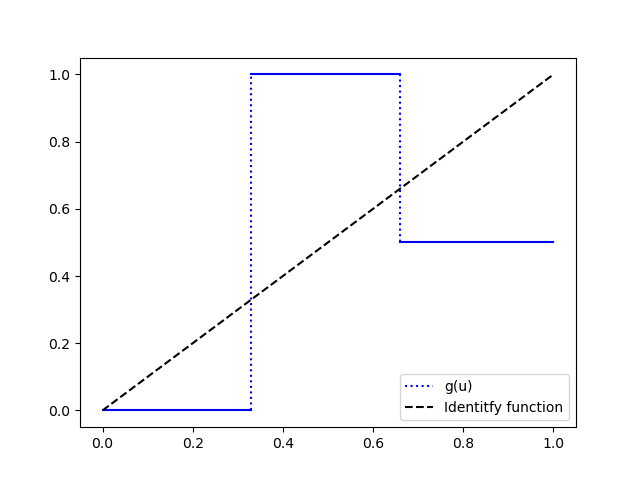
\includegraphics[width=.8\linewidth]{figures/fig1.png}
\end{figure}

Piecewise constant growth functions have been used in the studies of integro-difference equations; see for example~\cite{kot1, lut,otto,  pnas}. We rigorously construct periodic traveling waves with periodic speeds for (\ref{q}). To the best of our knowledge, this is the first time that traveling waves with oscillating speeds have been analytically established  for scalar spatiotemporal equations with constant parameters. We also show the convergence of solutions with compactly supported initial data to translations of the traveling wave under appropriate conditions. Equation (\ref{q}) may be viewed as a symbolic model for integro-difference equations with a growth function exhibiting a strong Allee effect and a period two cycle. The results obtained this paper provide important insights into integro-difference equations with general growth functions. 


%\section{Results}
\section{Periodic traveling waves}
%\subsection{Periodic traveling waves}

In this section, we construct a periodic traveling wave solution to the recurrence \eqref{q}. We will assume the dispersal kernel $k$ satisfies the following hypotheses:

\def\Hone{(\text{H1})}
\def\Htwo{(\text{H2})}
\def\Hthree{(\text{H3})}
\def\Hfour{(\text{H4})}

%\begin{hyp} \label{hypothesis1} The disperal kernel $k$ is Lebesgue measurable, and

\begin{enumerate}[(H1)]
\item $k$ is a non-negative, Lebesgue-integrable function with $\int_{-\infty}^{\infty} k(x) \, dx = 1$;

\item $k(x)=k(-x)$ for all $x\in\mathbb R$;

\item the support of $k$ is connected;

\item  for all $\lambda\in(0,1)$, for all $a\in\mathbb R$, the equation $k(x)=\lambda k(x-a)$ has at most one real solution.
\end{enumerate}


%\end{hyp}

%\begin{rem}
%Hypotheses (H1)-(H4) are scale-invariant, that is, if $k(x)$ satisfies (H1)-(H4), then so does $\hat{k}(x):=ak(ax)$ for any $a>0$. Thus, when checking the hypotheses for a particular dispersal kernel, we may rescale without loss of generality.
%\end{rem}

%\begin{prop} \label{prop1}
%%Let $\mathcal B$ denote the space of bounded, continuous, non-negative functions $\mathbb R \to \mathbb R$. $Q$ is a bounded nonlinear operator $\mathcal B \to \mathcal B$, and satisfies the following properties for all $u \in \mathcal B$:
%The operator $Q$ satisfies the following properties for all bounded continuous functions $u : \mathbb R \to \mathbb R_{\geq 0}$:
%
%\begin{enumerate}[(i.)]
%\item \it{(Translation invariance)} $Q[T^t[u]]=T^t[Q[u]]$ for any translation operator $T^t[u](x)=u(x+t)$.
%\item \it{(Symmetric)} If $u(x)=u(-x)$ then $Q[u](x)=Q[u](-x)$.
%\item \it{(Limit-preserving)} If $u(x)\to\ell$ as $x\to\infty$, then $Q[u](x)\to g(\ell)$ as $x\to\infty$; likewise as $x\to-\infty$.
%\end{enumerate}
%\end{prop}


\begin{lem} \label{lemmamain}
Let $w(x) = \int_x^\infty k(y) \, dy$. Define
\begin{equation}
c^* = \frac{1}{2} \sup \{ x\in\mathbb R | Q[\mtwo w](x) \geq \a \}
\end{equation}
Let $w_1(x) = w(x)$ and $w_2(x) = Q[w](x+c^*)$. If $|| w_2 ||_\infty \leq \b $, then $w_1$ and $w_2$ satisfy
\begin{equation} \label{lemma1claim1}
Q[w_1](x) = w_2(x-c^*)
\end{equation}
and
\begin{equation}\label{lemma1claim2}
Q[w_2](x) = w_1(x-c^*)
\end{equation}
for all $x \in \mathbb R$.
\end{lem}

%
%\begin{lem} \label{lemma0.5}
%$Q[w_1](x) = w_2(x)$ for all $x\in\mathbb R$.
%\end{lem}




\begin{proof}
Equation \ref{lemma1claim1} follows directly from the definition of $w_2(x)$.

To prove \ref{lemma1claim2}, observer that $w_1$ is monotonically decreasing with $w_1(-\infty)=\mtwo$ and $w_1(\infty)=0$. It follows that $w_1(x)>\b$ for $x<x_\b$, $\a\leq w_1(x)\leq\b$ for $x_\b\leq x\leq x_\a$, and $w_1(x)<\a$ for $x>x_\a$, where $x_a$ and $x_b$ are the solutions of
\begin{equation}
w_1(x_\a) = \a, \quad w_1(x_\b) = \b
\end{equation}
This yields
\begin{equation}
g(w_1(x)) = \begin{cases}
\m & x < x_\b \\
\mtwo & x_\b \leq x \leq x_\a \\
0 & x > x_\a
\end{cases}
\end{equation}
Applying the integro-difference operator yields
\begin{equation} \label{qw1calculation}
\begin{aligned}
Q[w_1](x) %&= \int_{-\infty}^{\infty} k(x-y) g(w_1(y)) \, dy \\
&= \m \int_{-\infty}^{x_\b} k(x-y) \, dy + \mtwo \int_{x_\b}^{x_\a} k(x-y) \, dy %\\
\end{aligned} \end{equation}
%&= \m \int_{x-x_\b}^{\infty} k(y) \, dy + \int_{x-x_\a}^{x-x_\b} k(y) \, dy \\
%&= \mtwo \int_{x-x_\a}^{\infty} k(y) \, dy - (\mtwo-\m) \int_{x-x_\b}^{\infty} k(y) \, dy \\
Using a substitution on both integrals yields equation \eqref{w2}, proving the first part of the lemma.
%It can now be seen that replacing $x$ with $x-c^*$ in equation \eqref{w2} produces \eqref{qw1calculation}.
%\end{proof}



%
%\begin{lem} \label{lemma0}
%$w_1(x)$ is monotone, while $w_2(x)$ has at most one turning point.
%\end{lem}
%
%
%
%
%\begin{proof}
%The monotonicity of $w_1$ follows since $w_1'(x)=-k(x)\leq 0$ by hypothesis (H1). To count the turning points of $w_2$, let $x_\a=\sup\{x\in\mathbb R\mid w_1(x)\geq\a\}$ and $x_\b=\sup\{x\in\mathbb R\mid w_1(x)\geq\b\}$. Since $w_1$ is monotone, it follows that $w_1(x)>\b$ for $x<x_\b$, $\a\leq w_1(x)\leq\b$ for $x_\b\leq x\leq x_\a$, and $w_1(x)<\a$ for $x>x_\a$. Applying the integro-difference operator to $w_1$ yields
%\begin{equation} \label{qw1calculation}
%\begin{aligned}
%Q[w_1](x) %&= \int_{-\infty}^{\infty} k(x-y) g(w_1(y)) \, dy \\
%&= \m \int_{-\infty}^{x_\b} k(x-y) \, dy + \int_{x_\b}^{x_\a} k(x-y) \, dy \\
%%&= \m \int_{x-x_\b}^{\infty} k(y) \, dy + \int_{x-x_\a}^{x-x_\b} k(y) \, dy \\
%&= \int_{x-x_\a}^{\infty} k(y) \, dy - (1-\m) \int_{x-x_\b}^{\infty} k(y) \, dy
%\end{aligned} \end{equation}
%
%Taking the derivative with respect to $x$, we find
%\begin{equation}\label{dw2dx}
%\frac{d}{dx}Q[w_1] = -k(x-x_\a) + (1-\m)k(x-x_\b)
%\end{equation}
%
%From hypothesis (H4), we can conclude that \eqref{dw2dx} has at most one zero-crossing, hence $w_2(x)$ has at most one turning point.
%\end{proof}


%
%Hypothesis (H1) implies $w_1$ and $w_2$ have well-defined limits at $\pm\infty$ given by $w_1(\infty)=w_2(\infty)=0$, $w_1(-\infty)=1$, and $w_2(-\infty)=\m$. Furthermore, $w_1$ is monotonically decreasing, while $w_2$ may be non-monotonic.


%\begin{lem} \label{lemma1}
%If $\sup_{x\in\mathbb R}w_2(x)\leq \b$, then $Q[w_2](x)=w_1(x-c^*)$ for all $x\in\mathbb R$.
%\end{lem}

%\begin{lem} \label{lemma1}
%If $ ||w_2||_\infty \leq \b$, then $Q[w_2](x)=w_1(x-c^*)$ for all $x\in\mathbb R$.
%\end{lem}

%'\begin{proof}
To prove the second half, we differentiate $w_2$ with respect to $x$:
\begin{equation} \label{dqw1}
\frac{dw_2}{dx} = \mtwo k(x-x_\a) - (\mtwo-\m) k(x-x_\b)
\end{equation}
A transformation of coordinates shows that equation \eqref{dqw1} is proportional to $k(x) - \frac{\mtwo-\m}{\mtwo} k(x+x_\a-x_\b)$; by hypothesis (H4), $\frac{dw_2}{dx}$ has at most one real zero.

It can be shown by cases that $w_2$ is either monotonically decreasing or has a unique turning point $x_0 \in \mathbb R$. In both cases, the curve $u=w_2(x)$ crosses the horizontal line $u=\a$ exactly once at the point $x=2c^*$. In the latter case, we utilize the assumption that $|| w_2 ||_\infty \leq \b$ . In all cases, 


%By Hypothesis (H4), we have assumed that the integrand on the right hand side has at most one zero. We can now proceed in cases. $w_2(x)$ has either zero or one turning point(s). In the first case, $w_2(x)$ is monotonically decreasing and satisfies $w_2(x) \geq \a$ for $x \leq 2c^*$ and $w_2(x) < \a$ for $x > 2c^*$. In the second case, $w_2(x)$ has a unique turning point $x_0 \in \mathbb R$; it follows that $w_2(x)$ is monotonically increasing on $(-\infty,x_0)$ and monotonically decreasing on $(x_0,\infty)$, and $x_0$ is a global maximum. By the assumption $w_2(x)\leq\beta$ for all $x$, we have $w_2(x_0)\leq\beta$. It follows that $c^* \in (\frac{x_0}{2},\infty)$, and $w_2(x)$ satisfies $g(w_2(x))=1$ for $x<2c^*$ and $g(w_2(x)) = 0$ for $x>2c^*$. In each case, we have
%%
\begin{equation}
g(w_2(x)) = \begin{cases}
1 & x \leq 2c^* \\
0 & x > 2c^*
\end{cases}
\end{equation}


%Let $x_\a=\sup\{x\in\mathbb R\mid w_1(x)\geq\a\}$ and $x_\b=\sup\{x\in\mathbb R\mid w_1(x)\geq\b\}$. Since $w_1$ is monotone, it follows that $w_1(x)>\b$ for $x<x_\b$, $\a\leq w_1(x)\leq\b$ for $x_\b\leq x\leq x_\a$, and $w_1(x)<\a$ for $x>x_\a$. Applying the integro-difference operator to $w_1$ yields
%\begin{equation} \label{qw1calculation}
%\begin{aligned}
%Q[w_1](x) &= \int_{-\infty}^{\infty} k(x-y) g(w_1(y)) \, dy \\
%&= \m \int_{-\infty}^{x_\b} k(x-y) \, dy + \int_{x_\b}^{x_\a} k(x-y) \, dy \\
%&= \m \int_{x-x_\b}^{\infty} k(y) \, dy + \int_{x-x_\a}^{x-x_\b} k(y) \, dy \\
%&= \int_{x-x_\a}^{\infty} k(y) \, dy - (1-\m) \int_{x-x_\b}^{\infty} k(y) \, dy
%\end{aligned} \end{equation}
%
%Taking the derivative with respect to $x$, we find
%\begin{equation}\label{dw2dx}
%\frac{d}{dx}Q[w_1] = -k(x-x_\a) + (1-\m)k(x-x_\b)
%\end{equation}

%From hypothesis (H4), we can conclude that \eqref{dw2dx} has at most one zero-crossing, hence $w_2(x)$ has at most one turning point. This leaves two cases:
%\begin{enumerate}[{Case} 1.]
%\item If $w_2$ has no turning points, it must be monotonically decreasing.
%\item If $w_2$ has a single turning point $x^*$, then $w_2(x)$ is increasing on $(-\infty,x^*)$ and decreasing on $(x^*,\infty)$, with $\m \leq w_2(x^*)\leq \b$.
%\end{enumerate}
%
%In both cases, $w_2(x)$ has a well-defined right inverse on the open interval $(0,\m)$. Since $0<\a<\m$, let
%\begin{equation}
%c^*=\frac{1}{2}\sup\{x\in\mathbb R\mid w_2(x)\geq\a\}
%\end{equation}

%It follows that $w_2(x)\geq\a$ for $x\leq 2c^*$ and $w_2(x)<\alpha$ for $x>2c^*$. Along with the assumption that $\sup_{x\in\mathbb R}w_2(x)\leq\b$, we can apply the integro-difference operator once more:
Thus,
\begin{equation} \begin{aligned}
Q[w_2](x) &= \int_{-\infty}^{\infty} k(x-y) g(w_2(y)) \, dy \\
&= \int_{-\infty}^{2c^*} k(x-y) \, dy \\
&= \int_{x-2c^*}^{\infty} k(y) \, dy \\
&= w_1(x-2c^*).
\end{aligned} \end{equation}
%By defining $c^* = \frac{1}{2}x_0$, and applying the integro-difference operator, we can see that $w_1$ and $w_2$ are both solutions to the periodic traveling wave equation with mean speed $c^*$:
%\begin{equation}
%Q^2[w_1](x) = w_1(x-2c^*); \quad Q^2[w_2](x) = w_2(x-2c^*)
%\end{equation}
\end{proof}


By Lemma \ref{lemmamain}, the wave functions $w_1(x)$ and $w_2(x)$ satisfy $Q^2[w_1](x)=w_1(x-2c^*)$ and $Q^2[w_2](x)=w_2(x-2c^*)$. As a result, they can be used to construct a solution which spreads in space with a mean speed of $c^*$ and alternates in shape every two time steps.

%\begin{cor} If $||w_2||_\infty \leq \beta$, then for all $x\in\mathbb R$,
%\begin{equation}
%Q^2[w_1](x) = w_1(x-2c^*)
%\end{equation}
%and
%\begin{equation}
%Q^2[w_2](x) = w_2(x-2c^*)
%\end{equation}
%\end{cor}


%The condition that $\sup_{x\in\mathbb R}w_2(x)\leq \b$ may be difficult to verify for some choices of dispersal kernel. Thus, we provide a sufficient condition for this assumption:
%\begin{lem} \label{lemma}
%Let $x_\a$ and $x_\b$ be as defined in Lemma \ref{lemma1}. If $k(x)$ is unimodal and
%$$ \m +  (1-\mu)\int_{-(x_\a-x_\b)/2}^{(x_\a-x_\b)/2} k (y) \, dy \leq \b $$
%then $\sup_{x\in\mathbb R}w_2(x) \leq \b$.
%\end{lem}
%
%\begin{proof}
%For all $x\in\mathbb R$, we have
%\begin{equation} \begin{aligned}
%w_2(x) &= \int_{-\infty}^{\infty} k(x-y) g(w_1(y)) \, dy  \\
%&\leq\int_{-\infty}^{\infty} k(x-y) (\m + (\m-1) \mathbf 1_{[x_\b,x_\a]}(y) )\, dy \\
%&= \m + \int_{-\infty}^{\infty} k(x-y) (\m-1) \mathbf 1_{[x_\b,x_\a]}(y) \, dy \\
%&= \m +  (1-\mu)\int_{x_\b}^{x_\a} k (x-y) \, dy .
%\end{aligned}
%\end{equation}
%
%Taking the maximum over all $x$, we may shift the function horizontally so that the bounds of integration are symmetric. Since $k(x)$ is unimodal, the integral is then maximized for $x=0$.
%\begin{equation} \begin{aligned}
%\sup_{x\in\mathbb R} w_2(x) &\leq \sup_{x\in\mathbb R} \left( \m +  (1-\mu)\int_{x_\b}^{x_\a} k (x-y) \, dy \right) \\
%&= \sup_{x\in\mathbb R} \left( \m +  (1-\mu)\int_{-(x_\a-x_\b)/2}^{(x_\a-x_\b)/2} k (x-y) \, dy \right) \\
%&= \m +  (1-\mu)\int_{-(x_\a-x_\b)/2}^{(x_\a-x_\b)/2} k (y) \, dy.
%\end{aligned}
%\end{equation}
%\end{proof}



\begin{thm} \label{theorem1}
Let $u_n(x)$ be a sequence of functions defined by
\begin{equation}
u_n(x) = \begin{cases} \label{ptw}
w_1(x-nc^*) & n \text{ even} \\
w_2(x-nc^*) & n \text{ odd}
\end{cases} \end{equation}
If $|| w_2 ||_\infty \leq \b $, then $u_n(x)$ satisfies $u_{n+1}(x) = Q[u_n](x)$ for all $n\geq 0$.
\end{thm}

\begin{proof}
Let $n \geq 0$. If $n$ is even, then $n+1$ is odd, so $u_n(x)=w_1(x-nc^*)$ and $u_{n+1}(x)=w_2(x-nc^*)$. Applying the integro-difference operator, we obtain
\begin{equation} \begin{aligned}
Q[u_n](x) &= Q[w_1](x-nc^*) \\
&= w_2(x-nc^*) \\
&= u_{n+1}(x)
\end{aligned} \end{equation}
by \eqref{w2}. On the other hand, if $n$ is odd, then $n+1$ is even, so $u_n(x)=w_2(x-nc^*+c^*)$ and $u_{n+1}(x)=w_1(x-nc^*-c^*)$. Applying the operator, we get
\begin{equation} \begin{aligned}
Q[u_n](x) &= Q[w_2](x-nc^*+c^*) \\
&= w_1(x-nc^*-c^*) \\
&= u_{n+1}(x)
\end{aligned} \end{equation}
by Lemma \ref{lemmamain}.
\end{proof}





The previous theorem shows that our model can exhibit a periodic traveling wave solution with alternating wave profiles. Furthermore, we derived a constant wave speed at which the oscillating pair of waves travels. We now turn our attention to the magnitude of the oscillation in the wave speed. For a sufficiently small $\ell > 0$, we may label the point of intersection of the curve $u=u_n(x)$ with the horizontal line $u=\ell$ by $\xi_{n,\ell}$, or simply $\xi_n$. It follows that $\xi_1,\xi_2,\xi_3,\dots\to\infty$ as $n\to\infty$; furthermore, the previous theorem implies that for any $\ell$, we have $\xi_{n+2}-\xi_n=2c^*$ for every $n\geq 1$.

$$
w_i(x) = \int_\Omega k(x-y+2c^*) g\left( \int_\Omega k(y-y') g(w_i(y')) \, dy' \right) \, dy
$$
For every $n\geq 1$, let $c_n = \xi_n - \xi_{n-1}$.

We now introduce an additional hypothesis for the spread of solutions with compactly supported initial condition.

Hypothesis 2. For sufficiently large $r_b$, with $r_a > r_b > 0$ and $\lambda \in (0,1)$, the equation

$$ k(x+r_a) - k(x-r_a) - \lambda k(x+r_b) + \lambda k(x-r_b) $$

has at most 3 solutions.

\begin{thm}  \label{theorem2}
If $||w_2|| \b$, then for all $\epsilon>0$, the sequence \ref{ptw} satisfies
\begin{equation}
\lim_{n\to\infty}\inf_{x<2n(c^*-\epsilon)}u_{2n}(x)=\mtwo
\end{equation}
and
\begin{equation}
\lim_{n\to\infty}\inf_{x<2n(c^*-\epsilon)}u_{2n+1}(x)=\m
\end{equation}
and 
\begin{equation}
\lim_{n\to\infty}\sup_{x>n(c^*+\epsilon)}u_n(x)=0.
\end{equation}
\end{thm}

\begin{proof}
\begin{equation} \begin{aligned}
\lim_{n\to\infty}\inf_{x<2n(c^*-\epsilon)}u_{2n}(x)
&= \lim_{n\to\infty}\inf_{x<2n(c^*-\epsilon)}w_1(x-2nc^*) \\
&= \lim_{n\to\infty}\inf_{x<-2n\epsilon}w_1(x) \\
&= \liminf_{x\to-\infty}w_1(x) \\ &= 1.
\end{aligned} \end{equation}

\begin{equation} \begin{aligned}
\lim_{n\to\infty}\inf_{x<2n(c^*-\epsilon)}u_{2n+1}(x)
&= \lim_{n\to\infty}\inf_{x<2n(c^*-\epsilon)}w_2(x-2nc^*) \\
&= \lim_{n\to\infty}\inf_{x<-2n\epsilon}w_2(x) \\
&= \liminf_{x\to-\infty}w_2(x) \\ &= \m.
\end{aligned} \end{equation}

\begin{equation} \begin{aligned}
\lim_{n\to\infty} \sup_{x>n(c^*+\epsilon)} u_n(x) 
&\leq \lim_{n\to\infty} \sup_{x>n(c^*+\epsilon)} \sup\{w_1(x-nc^*),w_2(x-nc^*)\} \\
&= \lim_{n\to\infty} \sup_{x>n\epsilon} \sup\{w_1(x),w_2(x)\} \\
&= \limsup_{x\to\infty} \sup\{w_1(x),w_2(x)\} \\ 
&= \sup\{\limsup_{x\to\infty} w_1(x),\limsup_{x\to\infty} w_2(x)\} \\
&= 0.
\end{aligned} \end{equation}
In the last calculation, the left hand side is known to be non-negative; therefore the limit is exactly equal to zero.
\end{proof}

\subsection{Spreading solutions}

\textbf{Note: this section contains incomplete results.}


In this section, we consider how the periodic traveling wave solutions in the preceding results correspond to solutions with a compactly supported initial population density. For simplicity, we restrict our attention to initial conditions where the maximum population value does not exceed the overcompensation threshold.

Let $\chi_{[-r,r]}$ denote the indicator function on $[-r,r]$. Suppose $u_0$ is a continuous function with compact support, and suppose $u_0$ satisfies $\a \leq u_0(x) \leq \b$ for $|x| \leq r$ and $u_0(x) < \a$ otherwise. It follows that
$$ g(u_0(x)) = \chi_{[-r,r]}(x) $$

%
%Let $u_n(x)$ be a sequence of continuous functions. For every $c \in \mathbb R$, define the sequence $a_n(x,c)$ by
%$$ a_n(x,c) = u_n(x+nc) $$
%Now, define
%$$ a(x,c) = \limsup_{n\to\infty} a_n(x,c). $$
%Note that since $a_n$ is bounded, this quantity must be finite. We say the rightware spreading speed of $u_0$ is defined by
%$$ c^*_+ = \inf \{ c \in \mathbb R \mid \lim_{x\to\infty} a(x,c) = 0 \} $$
%
%\begin{lem}
%If $||w_2||_\infty\leq\b$, the sequence \eqref{ptw} has a rightward spreading speed of $c^*$.
%\end{lem}
%
%\begin{proof}
%We have
%$$ a_n(x,c) = \begin{cases}
%w_1(x + n(c-c^*))  & n \text{ even} \\
%w_2(x + n(c-c^*)) & n \text{ odd}
%\end{cases} $$
%Thus,
%$$ \begin{aligned}
%a(x,c) &= \limsup_{n\to\infty} a_n(x,c) \\
%&= \limsup_{n\to\infty} \max \{ w_1(x + n(c-c^*)), w_2(x + n(c-c^*)) \} \\
%&= \begin{cases}
%1 & c < c^* \\
%\max\{w_1(x),w_2(x)\} & c=c^* \\
%0 & c>c^*
%\end{cases} \end{aligned} $$
%Taking the limit as $x\to\infty$,
%$$ a(\infty,c) = \begin{cases}
%1 & c < c^* \\
%0 & c \geq c^*
%\end{cases} $$
%\end{proof}



For a given $r \geq 0$, let $\phi(x,r) = \chi_{[-r,r]}(x)$, or simply $\phi_r$ for brevity. Define the operator $R[u] = g\left( Q[k*u](x) \right)$.

\begin{equation}
R[u](x) = g\left( \int k(x-y) g\left( \int k(y-z) u(z) \, dz \right) \, dy \right)
\end{equation}

\begin{lem}
Let $u_n(x)$ be a sequence of functions satisfying $u_{n+1}(x)=Q[u_n](x)$ for all $n \geq 0$ with initial condition $u_0 \in C(\mathbb R; [0,1])$. Then $u_{2n}(x) = (k*R^{n-1}[g\circ u])(x)$ for all $n\geq1 $.
\end{lem}

\begin{lem}
For sufficiently large $r \geq 0$, we have $R[\phi_r] = \phi_{r+\delta(r)}$, where $\delta(r)$ is a scalar function of $r$. It can be expressed as
$$ \delta(r) = \int R[\phi_r](x)  \, dx $$
\end{lem}

\begin{proof}
We have
$$ (k*\phi_r)(x) = K(x+r) - K(x-r) $$
Note that $(k*\phi_r)(0) = 2K(r)-1$, assuming a symmetryic dispersal kernel. Thus, assuming $\frac{d}{dx}(k*\phi_r)$ has at most one zero, a lower bound of $r \geq K^{-1}\left(\frac{\b+1}{2}\right)$ guarantees 
$$ R[\phi_r] = \begin{cases}
n_1 & |x| < r_1 \\
n_2 & r_1 \leq |x| \leq r_2 \\
0 & |x| > r_2
\end{cases} $$
\end{proof}
for some $r_2 > r_1 \geq 0$. 

Applying the convolution operator to this expression yields
$$ k*R[\phi_r] (x) = n_2 \int_{-r_2}^{r_2} k(x-y)\,dy - (n_2-n_1) \int_{-r_1}^{r_1} k(x-y) \, dy $$
$$ = n_2 \left[ K(x+r_2) - K(x-r_2)  \right] - (n_2-n_1) \left[ K(x+r_1) - K(x-r_1) \right] $$
Taking the derivative, we find
$$ \frac{d}{dx} \left[ k*R[\phi_r] \right] = n_2 \left[ k(x+r_2) - k(x-r_2)  \right] - (n_2-n_1) \left[ k(x+r_1) - k(x-r_1)\right] $$
We now require the following hypothesis on the disperal kernel:

(H5) For all $r_2>r_1>0$ and $\lambda \in (0,1)$, the equation
$$ k(x+r_2) - k(x-r_2) - \lambda k(x+r_1) + \lambda k(x-r_1) = 0 $$
has at most 3 solutions.

If hypothesis (H5) holds, we can then deduce that $k*R[\phi_r]$ has at most 3 turning points. This leaves only two cases: either $k*R[\phi_r]$ has a single turning point at $x=0$, or has 3 turning points, one at $x=0$, and two diametrically opposed turning points $+t$ and $-t$. In both cases, there is a unique $r_3>0$ satisfying $(k*R[\phi_r])(x) \geq \a$ for $|x| \leq r_3$ and $(k*R[\phi_r])(x) < \a$ otherwise. 

\textbf{Note: the above section contains unfinished proofs.}




\begin{figure}[h!] 
\centering
  \caption{Spreading behavior for a uniform dispersal kernel with $\alpha=0.3$, $\mu=0.6$, and $\beta=0.7$. The time steps corresponding to $w_1(x)$ are colored in blue, while time steps corresponding to $w_2(x)$ are colored in red.}
\label{fig5}
  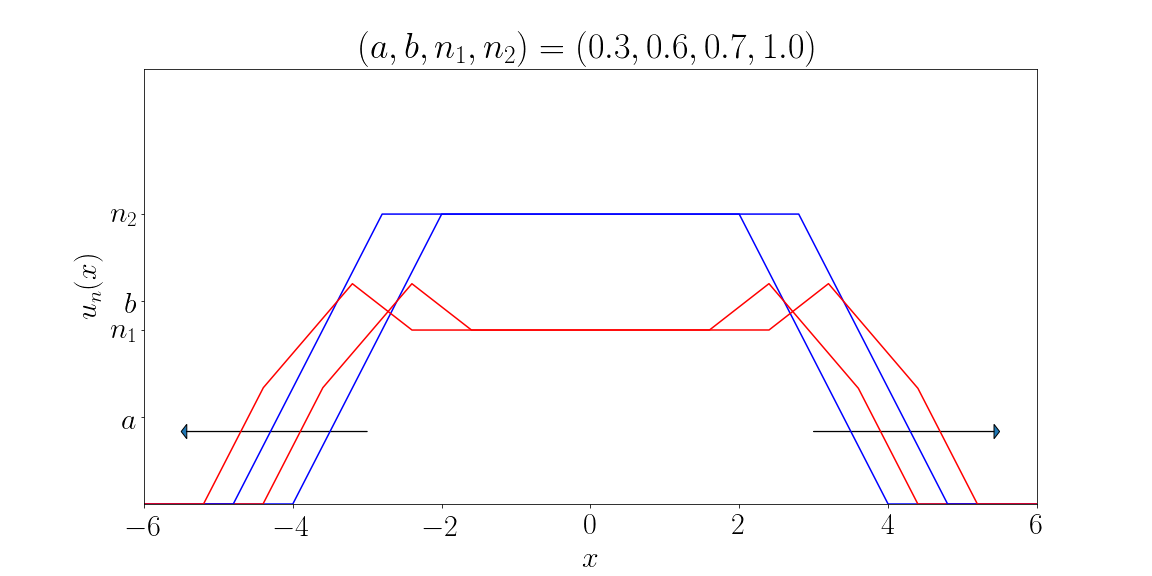
\includegraphics[width=.8\linewidth]{figures/fig5.png}
\end{figure}

\begin{rem}
This theorem indicates that a solution with proper compactly supported initial data coverges to translations of periodic traveling waves with profiles $w_1(x)$ and $w_2(x)$ in the positive direction and profiles $w_1(-x)$ and $w_2(-x)$ in the negative direction.
\end{rem}


\section{Examples}

In this section, we construct the periodic traveling wave solution for several well-known disperal kernels in population biology, namely the uniform, Laplace, and normal distributions. For the uniform and Laplace kernels, we were able to construct a piecewise expression for the mean wave speed in terms of the model parameters. 

\begin{ex}
The Laplace kernel is given by
\begin{equation}\label{laplacekernel}
k(x) = \frac{1}{2} e^{-|x|}
\end{equation}

The reader can easily verify that the Laplace kernel satisfies hypotheses (H1) - (H3); the proof of (H4) is left in the appendix \ref{laplaceproof}.

\begin{figure}
\centering
\begin{subfigure}{.5\textwidth}
  \centering
  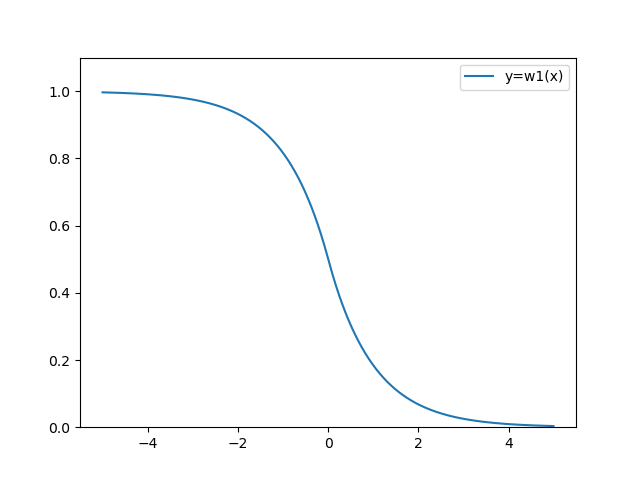
\includegraphics[width=.9\linewidth]{figures/fig2A.png}
  \label{fig:sub1}
\end{subfigure}%
\begin{subfigure}{.5\textwidth}
  \centering
  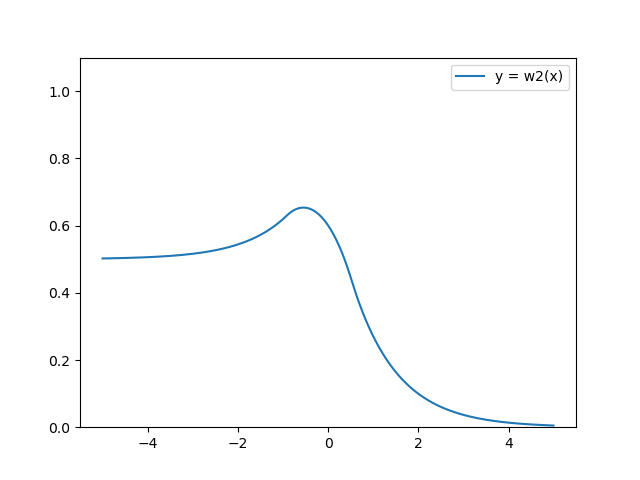
\includegraphics[width=.9\linewidth]{figures/fig2B.png}
  \label{fig:sub2}
\end{subfigure}
\caption{The shape of the two periodic traveling wave profiles with Laplace dispersal kernel and growth parameters $\a=0.3$, $\m=0.5$, and $\b=0.8$.}
\label{fig:test}
\end{figure}


The periodic traveling wave profiles are given by

\begin{equation} \label{w1laplace}
w_1(x) =   \begin{cases} 
n_2 - \frac{1}{2} n_2 e^{x} & x \leq 0 \\
\frac{1}{2} n_2 e^{-x} & x > 0
\end{cases}
\end{equation}
and
%\begin{equation}\label{laplacew2}
%w_2(x) = \begin{cases}
%m - \frac{1}{2} e^{x - \alpha} + \frac{1-\m}{2} e^{x - \beta} & x < \beta \\
%1 - \frac{1}{2} e^{x-\alpha} - \frac{1-\m}{2} e^{-(x-\beta)} & \beta \leq x \leq \alpha \\
%\frac{1}{2} e^{-(x-\alpha)} - \frac{1-\m}{2} e^{-(x-\beta)} & x > \alpha
%\end{cases}
%\end{equation}
%\begin{equation} \label{w2laplace}
%w_2(x) = \begin{cases}
%m + C_1 e^x & x < x_\b \\
%1 - C_2 e^x - C_3 e^{-x} & x_\b \leq x \leq x_\a \\
%C_4 e^{-x} & x_\a < x 
%\end{cases} \end{equation}
%or equivalently

\begin{equation} \label{w2laplace}
w_2(x) = \begin{cases}
\m + \left( \frac{1}{2}(\mtwo-\m)e^{-x_\b} - \frac{1}{2}\mtwo e^{-x_\a} \right) e^x & x < x_\b \\
\mtwo - \frac{1}{2} \mtwo e^{-x_\a} e^x - \frac{1}{2} (\mtwo-\m) e^{x_\b}   e^{-x} & x_\b \leq x \leq x_\a \\
\left( \frac{1}{2} \mtwo e^{x_\a} - \frac{1}{2}\mtwo(\mtwo-\m) e^{x_\b} \right) e^{-x} & x_\a < x 
\end{cases} \end{equation}

with $x_a = F(a)$, $x_b=F(b)$, and
\begin{equation}
F(p) = \begin{cases} -\ln(2p) &p \leq \frac{1}{2} \\ \ln(2-2p) & p > \frac{1}{2} \end{cases}
\end{equation}

\begin{figure}[h!] 
\centering
  \caption{Numerical simulation of our model using the Laplace dispersal kernel. The parameters chosen for this simulation were $\a=0.2$, $\m=0.3$, and $\b=0.8$, and $\mtwo=1.0$. Later timepoints are colored in red, with earlier timepoints colored in green.}
\label{fig3}
  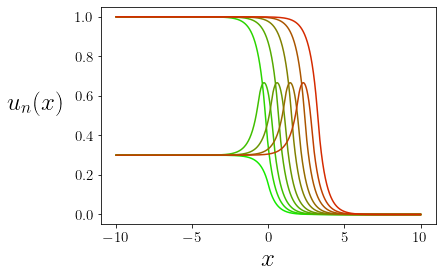
\includegraphics[width=.8\linewidth]{figures/fig3.png}
\end{figure}


A necessary condition for formulas \eqref{w1laplace} and \eqref{w2laplace} to generate a periodic traveling wave solution are given in Lemma \ref{laplacebound}. This leads to an equation for the mean wave speed
\begin{equation}
c^* = \begin{cases}
\frac{1}{2} \log \left( \frac{1}{2\a} \mtwo e^{x_\a} - \frac{1}{2\a}(\mtwo-\m)e^{x_\b} \right) & \a \leq w_2(x_\a) \\
\frac{1}{2} \log \left( \frac{1}{\mtwo} e^{-x_\a} \left( \m - \a + \sqrt{(\m-\a)^2-\mtwo(\mtwo-\m)e^{x_\b-x_\a}}\right)\right) & w_2(x_\a) < \a < w_2(x_\b) \\
\frac{1}{2} \log \left( \frac{2(\a-\m)}{(\mtwo-\m)\exp(-x_\b)-\mtwo \exp(-x_\a)}\right) & \a \geq w_2(x_\b)
\end{cases} 
\end{equation}
%and
%
%\begin{equation} \begin{aligned}
%C_1 &= \frac{1-\m}{2}e^{-x_\b} - \frac{1}{2}e^{-x_\a} \\
%C_2 &= \frac{1}{2} e^{-x_\a} \\
%C_3 &= \frac{1-\m}{2} e^{x_\b} \\
%C_4 &= \frac{1}{2} e^{x_\a} - \frac{1-\m}{2} e^{x_\b}
%\end{aligned} \end{equation}
%
%%$x_\a=w_1^{-1}(\a)$, $x_\b=w_1^{-1}(\b)$, with
%%$$ w_1^{-1}(p) = \begin{cases} -\ln(2p) & p\leq \frac{1}{2} \\ \ln(2-2p) & p > \frac{1}{2} \end{cases} $$
%The constants $C_1,C_2,C_3$, and $C_4$ are continuous functions of the growth parameters $\alpha$, $\beta$, and $\mu$, with $C_2,C_3,C_4\geq0$. They can be expressed as piecewise expressions:
\newcommand{\Conecaseone}{\b(1-\m)-\a}
\newcommand{\Conecasetwo}{\frac{1-\m-4\a(1-\b)}{4(1-\b)}}
\newcommand{\Conecasethree}{- \frac{1-\b+\m(1-\a)}{4(1-\a)(1-\b)} }
%
%\begin{equation}
%C_1 = \begin{cases}
%\Conecaseone & \a,\b \leq \frac{1}{2} \\
%\Conecasetwo & \a\leq\frac{1}{2}<\b \\
%\Conecasethree & \frac{1}{2}<\a,\b
%\end{cases} \end{equation}
%
\newcommand{\Ctwocaseone}{\a}
\newcommand{\Ctwocasetwo}{\frac{1}{4(1-\a)}}
%
%\begin{equation}
%C_2 = \begin{cases}
%\Ctwocaseone & \a \leq \frac{1}{2} \\
%\Ctwocasetwo & \a > \frac{1}{2}
%\end{cases} \end{equation}
%
\newcommand{\Cthreecaseone}{\frac{1-\m}{4\b}}
\newcommand{\Cthreecasetwo}{(1-\m)(1-\b)}
%
%\begin{equation}
%C_3 = \begin{cases}
%\Cthreecaseone & \b \leq \frac{1}{2} \\
%\Cthreecasetwo & \b > \frac{1}{2}
%\end{cases} \end{equation}
%
\newcommand{\Cfourcaseone}{\frac{\b-\a(1-m)}{4\a\b}}
\newcommand{\Cfourcasetwo}{\frac{1-4\a(1-\m)(1-\b)}{4\a}}
\newcommand{\Cfourcasethree}{1-\a-(1-\m)(1-\b)}
%
%\begin{equation}
%C_4 = \begin{cases}
%\Cfourcaseone & \a,\b \leq \frac{1}{2} \\
%\Cfourcasetwo & \a\leq\frac{1}{2}<\b \\
%\Cfourcasethree & \frac{1}{2}<\a,\b
%\end{cases} \end{equation}
%
%To find $c^*$, we can now condition on the values of $w_2(x_\a)$ and $w_2(x_\b)$.
%
%\begin{enumerate}[{Case} 1.]
%\item If $w_2(x_\alpha)=C_4e^{-x_\a}>\a$, then $2c^*$ lies on the third piece of \eqref{w2laplace}. Hence the mean wave speed is given by $c^*=\frac{1}{2}\ln(\frac{C_4}{\a})$.
%
%\item If $w_2(x_\a)=C_4e^{-x_\a}\leq\a$ and $w_2(x_\b)=\m+C_1e^{x_\b}\geq\a$, then we solve the equation
%
%$$ 1 - C_2e^{2c^*} - C_3e^{-2c^*} = \a $$
%
%Multiplying through by $e^{2c^*}$ yields a quadratic in $e^{2c^*}$:
%
%$$ C_2 e^{4c^*} + (a-1) e^{2c^*} + C_3 = 0 $$
%
%Using the quadratic formula, we get two solutions to this equation. To determine which is correct, note that $w_2'(2c^*)$ must be negative. Since $C_2,C_3$ are negative, $w_2(x)$ is concave down on $[x_\b,x_\a]$, thus $w_2$ is increasing through the first solution and decreasing through the second. Clearly we must take the greater solution. Thus,
%$$ c^* = \frac{1}{2} \ln \left( \frac{1-\a + \sqrt{(1-\a)^2 - 4C_2C_3}}{2C_2} \right) $$
%
%\item If  $w_2(x_\b)=\m+C_1e^{x_\b}<\a$, we have
%
%$$ \m + C_1 e^{2c^*} = \a $$
%implies
%$$ c^* = \frac{1}{2} \ln \frac{\a-\m}{C_1} $$
%\end{enumerate}
%
%Our general formula is thus
%\begin{equation}
%c^* = \begin{cases}
%\frac{1}{2} \ln \left( \frac{C_4}{\a} \right) & \a<C_4e^{-x_\a} \\
%\frac{1}{2} \ln \left( \frac{1-\a + \sqrt{(1-\a)^2 - 4C_2C_3}}{2C_2} \right) & C_4e^{-x_\a}<\a<\m+C_1e^{x_\b} \\
%\frac{1}{2} \ln \left( \frac{\a-\m}{C_1}\right) & \a>\m+C_1e^{x_\b}
%\end{cases}
%\end{equation}
%We can write this formula more explicitly depending on the signs of $\a-\frac{1}{2}$ and $\b-\frac{1}{2}$ respectively.
%Let $c_1$ and $c_2$ denote the intermediate wave speeds measured at some threshold $0<h<m$. For this analysis we chose the threshold of $h=a$. Thus $c_1 = w_2^{-1}(a) - w_1^{-1}(a)=2c^*-\alpha$, and $c_2=2c^*+\alpha-c_1=2\alpha$. We can now define the relative fluctuation in wavespeed by
%
%$$ f = \frac{|c_1-c_2|}{c^*} = \frac{|2c^*-3\alpha|}{c^*} $$
%
%We can also consider
%
%$$ f^2 = \frac{(c_1-c_2)^2}{(c^*)^{2}} $$
%
%The derivative is
%
%$$ \frac{df^2}{da} = \frac{d}{da}(c_1-c_2)^2\frac{1}{(c^*)^2} $$
%
%$$ = 2(c_1-c_2)(\frac{dc_1}{da}-\frac{dc_2}{da})(c^*)^{-2} - 2(c_1-c_2)^2(c^*)^{-3} $$
%
%$$ = \frac{2(c_1-c_2)}{(c^*)^2}\left((\frac{dc_1}{da}-\frac{dc_2}{da}) - \frac{c_1-c_2}{c^*}\right) $$
%
%It follows that $f$ is differentiable with respect to all the parameters almost everywhere. We conjecture that
%
%$$ \frac{df}{da} \geq 0 , \quad \text{almost everywhere} $$
%
%We will first consider the case $a,b<\frac{1}{2}$, and $a<C_4e^{-\alpha}$. We then have $\alpha=-\ln(2a)$, $c^*=\frac{1}{2}\ln\frac{b-(1-m)a}{4a^2b}$ so that
%
%$$ f = \frac{|\ln\frac{b-(1-m)a}{4a^2b}+3\ln(2a)|}{\ln\frac{b-(1-m)a}{4a^2b}} $$
%$$ = \frac{|\ln(2a(b-(1-m)a))-\ln(b)|}{\ln(b-(1-m)a)-\ln(4a^2b)}  $$

Our formula can be written more explicitly based on the values of $\a$ and $\b$:
\begin{enumerate}[{Case} 1.]

\item $\a\leq\frac{1}{2}$, $\b\leq\frac{1}{2}$.
\begin{equation}
w_2(x) = \begin{cases}
\m + (\Conecaseone) e^x  & x < -\ln(2\b) \\
1 - \Ctwocaseone e^x - \Cthreecaseone e^{-x} & -\ln(2\b) < x < -\ln(2\a) \\
\Cfourcaseone e^{-x} & x > -\ln(2\a)
\end{cases}
\end{equation}

We have $w_2(x_\a)=\frac{\b-\a(1-\m)}{2\b}$ and $w_2(x_\b)=\m + \frac{\b(1-\m)-\a}{2\b}$. Thus,
\begin{equation}
c^* = \begin{cases}
\frac{1}{2} \ln \left( \frac{\b-\a(1-\m)}{4\a^2\b} \right) & \a < \frac{\b-\a(1-\m)}{2\b} \\
\frac{1}{2} \ln \left( \frac{1-\a + \sqrt{(1-\a)^2 - \frac{\a(1-\m)}{\b}}}{2\a} \right) & \frac{\b-\a(1-\m)}{2\b} \leq \a \leq \frac{\b(1+\m)-\a}{2\b} \\
\frac{1}{2} \ln \left( \frac{\a-\m}{\b(1-\m)-\a}\right) & \a > \frac{\b(1+\m)-\a}{2\b}
\end{cases}
\end{equation}


\item $\a\leq\frac{1}{2}$, $\b>\frac{1}{2}$.
\begin{equation}
w_2(x) = \begin{cases}
\m + \Conecasetwo e^x  & x < \ln(2-2\b) \\
1 - \Ctwocaseone e^x - \Cthreecasetwo e^{-x} & \ln(2-2\b) < x < -\ln(2\a) \\
\Cfourcasetwo e^{-x} & x > -\ln(2\a)
\end{cases}
\end{equation}

We have $w_2(x_\a)=\frac{1-4\a(1-\m)(1-\b)}{2}$ and $w_2(x_\b)=\frac{1+\m-4\a(1-\b)}{2}$. Thus,
\begin{equation}
c^* = \begin{cases}
\frac{1}{2} \ln \left( \frac{1-4\a(1-\m)(1-\b)}{4\a^2} \right) & a<\frac{1-4\a(1-\m)(1-\b)}{2} \\
\frac{1}{2} \ln \left( \frac{1-\a + \sqrt{(1-\a)^2 - 4\a(1-\m)(1-\b)}}{2\a} \right) & \frac{1-4\a(1-\m)(1-\b)}{2}\leq\a\leq\frac{1+\m-4\a(1-\b)}{2} \\
\frac{1}{2} \ln \left( \frac{4(\a-\m)(1-\b)}{1-\m-4\a(1-\b)}\right) & \a>\frac{1+\m-4\a(1-\b)}{2}
\end{cases}
\end{equation}


\item $\a>\frac{1}{2}$, $\b>\frac{1}{2}$.
\begin{equation}
w_2(x) = \begin{cases}
\m \Conecasethree e^x  & x < \ln(2-2\b) \\
1 - \Ctwocasetwo e^x - \Cthreecasetwo e^{-x} & \ln(2-2\b) < x < \ln(2-2\a) \\
(\Cfourcasethree) e^{-x} & x > \ln(2-2\a)
\end{cases}
\end{equation}

Thus, $w_2(x_\a)=\frac{1-\a-(1-\m)(1-\b)}{2(1-\a)}$ and $w_2(x_\b)=\m - \frac{1-\b+\m(1-\a)}{2(1-\a)}$

\begin{equation}
c^* = \begin{cases}
\frac{1}{2} \ln \left( \frac{1-\a-(1-\m)(1-\b)}{\a} \right) & \a<\frac{1-\a-(1-\m)(1-\b)}{2(1-\a)} \\
\frac{1}{2} \ln \Big( 2(1-\a)\left[1-\a + \sqrt{\frac{(1-\a)^3-(1-\m)(1-\b) }{1-\a}}\right] \Big) & \frac{1-\a-(1-\m)(1-\b)}{2(1-\a)}\leq\a\leq\frac{\b-1+\m(1-\a)}{2(1-\a)} \\
\frac{1}{2} \ln \left( \frac{4(\m-\a)(1-\a)(1-\b)}{1-\b+\m(1-\a)}\right) & \a>\frac{\b-1+\m(1-\a)}{2(1-\a)}
\end{cases}
\end{equation}

\end{enumerate}

%%%%%%%%%%%%%%%%%%%%%%%%%%%%%%%%%%%%%%%%%%%%%%%%
%They are given explicitly by
%
%\renewcommand{\Conecaseone}{\b\m'-\a}
%\renewcommand{\Conecasetwo}{\frac{\m'-4\a\b'}{4\b'}}
%\renewcommand{\Conecasethree}{- \frac{\b'+\m\a'}{4\a'\b'} }
%
%\begin{equation}
%C_1 = \begin{cases}
%\Conecaseone & \a,\b < \frac{1}{2} \\
%\Conecasetwo & \a<\frac{1}{2}<\b \\
%\Conecasethree & \frac{1}{2}<a,b
%\end{cases} \end{equation}
%
%\renewcommand{\Ctwocaseone}{\a}
%\renewcommand{\Ctwocasetwo}{\frac{1}{4\a'}}
%
%\begin{equation}
%C_2 = \begin{cases}
%\Ctwocaseone & \a < \frac{1}{2} \\
%\Ctwocasetwo & \a > \frac{1}{2}
%\end{cases} \end{equation}
%
%\renewcommand{\Cthreecaseone}{\frac{\m'}{4\b}}
%\renewcommand{\Cthreecasetwo}{\m'\b'}
%
%\begin{equation}
%C_3 = \begin{cases}
%\Cthreecaseone & \b < \frac{1}{2} \\
%\Cthreecasetwo & \b > \frac{1}{2}
%\end{cases} \end{equation}
%
%\renewcommand{\Cfourcaseone}{\frac{\b-\a\m'}{4\a\b}}
%\renewcommand{\Cfourcasetwo}{\frac{1-4\a\m'\b'}{4\a}}
%\renewcommand{\Cfourcasethree}{\a'-\m'\b'}
%
%\begin{equation}
%C_4 = \begin{cases}
%\Cfourcaseone & \a,\b < \frac{1}{2} \\
%\Cfourcasetwo & \a<\frac{1}{2}<\b \\
%\Cfourcasethree & \frac{1}{2}<a,b
%\end{cases} \end{equation}
%
%To find $c^*$, we can now condition on the values of $w_2(\alpha)$ and $w_2(\beta)$.
% If $w_2(\alpha)=C_4e^{-\alpha}>a$, then we know $x_a>\alpha$, so that $C_4e^{-x_a}=C_4e^{-2c^*}=a$ implies $c^*=\frac{1}{2}\ln(\frac{C_4}{a})$.
%
%If $w_2(\alpha)<a$ and $w_2(\beta)>a$, then we solve the equation
%
%$$ 1 - C_2e^x - C_3e^{-x} = a $$
%
%Multiplying through by $e^x$ yields a quadratic in $e^x$:
%
%$$ e^x - C_2e^{2x} - C_3 = ae^x $$
%
%$$ C_2 e^{2x} + (a-1) e^x + C_3 = 0 $$
%
%$$ e^x = \frac{1-a \pm \sqrt{(1-a)^2 - 4C_2C_3}}{2C_2} $$
%
%Since $C_2,C_3$ are negative, we know the function is concave down on this piece. Therefore, we take the rightmost solution, since the curve must be increasing through this point since the solution is unique.
%
%$$ c^* = \frac{1}{2} \ln \left( \frac{1-a + \sqrt{(1-a)^2 - 4C_2C_3}}{2C_2} \right) $$
%
%In the final case where $w_2(\beta)<a$, we have
%
%$$ m + C_1 e^{x_a} = a $$
%implies
%$$ C_1e^{x_a} = a-m$$
%$$ x_a = \ln \frac{a-m}{C_1} $$
%$$ c^* = \frac{1}{2} \ln \frac{a-m}{C_1} $$
%
%%Our general formula is thus
%\begin{equation}
%c^* = \begin{cases}
%\frac{1}{2} \ln \left( \frac{C_4}{a} \right) & a<w_2(\alpha) \\
%\frac{1}{2} \ln \left( \frac{\a' + \sqrt{\a'^2 - 4C_2C_3}}{2C_2} \right) & w_2(\alpha)<a<w_2(\beta) \\
%\frac{1}{2} \ln \left( \frac{a-m}{C_1}\right) & a>w_2(\beta)
%\end{cases}
%\end{equation}
%
%Since the form of $w_2(x)$, and thus of $c^*$, depends on the values of $\a$ and $\b$; thus we will split into three cases for further analysis.
%
%\begin{enumerate}[{Case} 1.]
%
%\item $\a<\frac{1}{2}$, $\b<\frac{1}{2}$.
%\begin{equation}
%w_2(x) = \begin{cases}
%\m + (\Conecaseone) e^x  & x < -\ln(2\b) \\
%1 - \Ctwocaseone e^x - \Cthreecaseone e^{-x} & -\ln(2\b) < x < -\ln(2\a) \\
%\Cfourcaseone e^{-x} & x > -\ln(2\a)
%\end{cases}
%\end{equation}
%
%We have $w_2(\alpha)=\frac{\b-\a\m'}{2\b}$ and $w_2(\beta)=\m + \frac{\b\m'-\a}{2\b}$. Thus,
%\begin{equation}
%c^* = \begin{cases}
%\frac{1}{2} \ln \left( \frac{\b-\a\m'}{4\a^2\b} \right) & \a < \frac{\b-\a\m'}{2\b} \\
%\frac{1}{2} \ln \left( \frac{\a'+ \sqrt{\a'^2 - \frac{\a\m'}{b}}}{2\a} \right) & \frac{\b-\a\m'}{2\b} < a < \m + \frac{\b\m'-\a}{2\b} \\
%\frac{1}{2} \ln \left( \frac{a-m}{\b\m'-\a}\right) & a > \m + \frac{\b\m'-\a}{2\b}
%\end{cases}
%\end{equation}
%
%
%\item $\a<\frac{1}{2}$, $\b>\frac{1}{2}$.
%\begin{equation}
%w_2(x) = \begin{cases}
%\m + \Conecasetwo e^x  & x < \ln(2\b') \\
%1 - \Ctwocaseone e^x - \Cthreecasetwo e^{-x} & \ln(2\b') < x < -\ln(2\a) \\
%\Cfourcasetwo e^{-x} & x > -\ln(2\a)
%\end{cases}
%\end{equation}
%
%We have $w_2(\alpha)=\frac{1-4\a\b'\m'}{2}$ and $w_2(\beta)=\frac{1+\m-4\a\b'}{2}$. Thus,
%\begin{equation}
%c^* = \begin{cases}
%\frac{1}{2} \ln \left( \frac{1-4\a\b'\m'}{4\a^2} \right) & a<\frac{1-4\a\b'\m'}{2} \\
%\frac{1}{2} \ln \left( \frac{\a' + \sqrt{\a'^2 - 4\a\b'\m'}}{2\a} \right) & \frac{1-4\a\b'\m'}{2}<a<\frac{1+\m-4\a\b'}{2} \\
%\frac{1}{2} \ln \left( \frac{4\b'(a-m))}{\m'-4\a\b'}\right) & a>\frac{1+\m-4\a\b'}{2}
%\end{cases}
%\end{equation}
%
%
%\item $\a>\frac{1}{2}$, $\b>\frac{1}{2}$.
%\begin{equation}
%w_2(x) = \begin{cases}
%\m \Conecasethree e^x  & x < \ln(2\b') \\
%1 - \Ctwocasetwo e^x - \Cthreecasetwo e^{-x} & \ln(2\b') < x < \ln(2\a') \\
%(\Cfourcasethree) e^{-x} & x > \ln(2\a')
%\end{cases}
%\end{equation}
%
%Thus, $w_2(\alpha)=\frac{\a'-\b'\m'}{2\a'}$ and $w_2(\beta)=\m - \frac{\b'+\a'\m}{2\a'}$
%
%\begin{equation}
%c^* = \begin{cases}
%\frac{1}{2} \ln \left( \frac{\a'-\b'\m'}{a} \right) & a<\frac{\a'-\b'\m'}{2\a'} \\
%\frac{1}{2} \ln \left( 2\a'^2 + 2\a'\sqrt{\a'^2 - \frac{\b'\m'}{\a'}} \right) & \frac{\a'-\b'\m'}{2\a'}<a<\m - \frac{\b'+\a'\m}{2\a'} \\
%\frac{1}{2} \ln \left( \frac{4\a'\b'(m-a)}{\b'+\a'\m}\right) & a>\m - \frac{\b'+\a'\m}{2\a'}
%\end{cases}
%\end{equation}
%
%\end{enumerate}
%%%%%%%%%%%%%%%%%%%%%%%%%%%%%%%%%%%%%%%%%%%%%%%%%%
%
%Each of the preceding cases can be generalized as follows:
%
%\begin{equation}
%w_2(x) = \begin{cases}
%m + C_1 e^x & x < \beta \\
%1 - C_2 e^x - C_3 e^{-x} & \beta < x < \alpha \\
%C_4 e^{-x} & \alpha < x 
%\end{cases} \end{equation}
%with 
%
%Note that $C_2$ and $C_3$ are strictly negative. 
%
%To find $c^*$, we can now condition on the values of $w_2(\alpha)$ and $w_2(\beta)$. If $w_2(\alpha)=C_4e^{-\alpha}>a$, then we know $x_a>\alpha$, so that $C_4e^{-x_a}=C_4e^{-2c^*}=a$ implies $c^*=\frac{1}{2}\ln(\frac{C_4}{a})$.
%
%If $w_2(\alpha)<a$ and $w_2(\beta)>a$, then we solve the equation
%
%$$ 1 - C_2e^x - C_3e^{-x} = a $$
%
%Multiplying through by $e^x$ yields a quadratic in $e^x$:
%
%$$ e^x - C_2e^{2x} - C_3 = ae^x $$
%
%$$ C_2 e^{2x} + (a-1) e^x + C_3 = 0 $$
%
%$$ e^x = \frac{1-a \pm \sqrt{(1-a)^2 - 4C_2C_3}}{2C_2} $$
%
%Since $C_2,C_3$ are negative, we know the function is concave down on this piece. Therefore, we take the rightmost solution, since the curve must be increasing through this point since the solution is unique.
%
%$$ c^* = \frac{1}{2} \ln \left( \frac{1-a + \sqrt{(1-a)^2 - 4C_2C_3}}{2C_2} \right) $$
%
%In the final case where $w_2(\beta)<a$, we have
%
%$$ m + C_1 e^{x_a} = a $$
%implies
%$$ C_1e^{x_a} = a-m$$
%$$ x_a = \ln \frac{a-m}{C_1} $$
%$$ c^* = \frac{1}{2} \ln \frac{a-m}{C_1} $$
%
%Our general formula is thus
%\begin{equation}
%c^* = \begin{cases}
%\frac{1}{2} \ln \left( \frac{C_4}{a} \right) & a<w_2(\alpha) \\
%\frac{1}{2} \ln \left( \frac{1-a + \sqrt{(1-a)^2 - 4C_2C_3}}{2C_2} \right) & w_2(\alpha)<a<w_2(\beta) \\
%\frac{1}{2} \ln \left( \frac{a-m}{C_1}\right) & a>w_2(\beta)
%\end{cases}
%\end{equation}
%
%Let $x_a=w_2^{-1}(a)$ (well-defined by Lemma 1.2). We can check which piece $x_a$ lies on by evaluating $w_2(x)$ at $x=\alpha$ and $x=\beta$.
%
%
%Since $w_2$ is increasing for $x<\log(2a)$, we know the solution to $w_2(x)=a$ must lie on the second or third pieces. This can be determined by checking the sign of $w_2(\log(2b))-a$. If it is positive, the horizontal line $y=a$ intersects the curve $y=w_2(x)$ on the third piece, and the solution can be found by solving $(mb+b-a)e^{-x}=a$. Otherwise, if the sign is negative, the solution occurs on the second piece as the solution to the equation
%
%$$ w_2(x)=a \iff m + 1 - \frac{m+1}{4b} e^x - ae^{-x} = a $$
%
%First let us group like terms and multiply by $4b$:
%
%$$ (m+1) e^x + (m + 1 - a) - 4abe^{-x} = 0 $$
%
%Using the substitution $y=e^x$, this equation becomes a quadratic in $y$:
%
%$$ (m+1) y^2 + (m + 1 - a) y - 4ab = 0 $$
%
%The solution is
%
%$$ y = \frac{a-m-1 \pm \sqrt{(m+1-a)^2 + 16ab(m+1)}}{2m+2}$$
%
%We know the global maximum of $w_2(x)$ lies somewhere in the open interval $(\log(2a),\log(2b))$, therefore we take the greater solution so that
%
%$$ c^* = \frac{1}{2} \log\left(  \frac{a-m-1 + \sqrt{(m+1-a)^2 + 16ab(m+1)}}{2m+2} \right) $$
%
%Then we can obtain the critical wave speed in two cases:
%$$ c^* = \begin{cases} \displaystyle
%\frac{1}{2} \log \left( \frac{mb+b-a}{a} \right) & m \geq \frac{2ab+a-b}{b} \\
%\displaystyle
% \frac{1}{2} \log\left(  \frac{a-m-1 + \sqrt{(m+1-a)^2 + 16ab(m+1)}}{2m+2} \right) & m < \frac{2ab+a-b}{b}
%\end{cases} $$
%
%Case 2: $a<\frac{1}{2}<b$. Then
%$$ w_2(x) = \int_{x+\log(2-2b)}^{\infty} \frac{m}{2}e^{-|y|}\,dy + \int_{x+\log(2-2b)}^{x-\log(2a)} \frac{1}{2}e^{-|y|} \,dy $$
%
%Then
%
%$$ w_2(x) = \frac{m}{2} - \frac{m+1}{2}\left( \min(\frac{e^{-x}}{2-2b},1) - \min((2-2b)e^{x},1) \right) - \frac{1}{2} \left( \min(2ae^{-x},1) - \min(\frac{1}{2a}e^{x},1) \right) $$
%
%so
%
%$$ w_2(x) = \begin{cases}
%\displaystyle
%m - \frac{4a(m+1)(1-b)-1}{4a} e^x & x <\log(2a) \\
%\displaystyle
%m+1 - (m+1)(a-b) e^x - ae^{-x} & \log(2a) \leq x \leq -\log(2-2b) \\
%\displaystyle
%\frac{m+1-4a(1-b)}{4(1-b)} e^{-x}  & x > -\log(2-2b)
%\end{cases} $$

\end{ex}

\begin{ex} Consider the Gaussian kernel with zero mean and unit variance given by
$$ k(x) = \frac{1}{\sqrt{2\pi}} e^{-\frac{x^2}{2}} $$
The kernel is symmetric and has connected support, hence it satisfies hypotheses (H1)-(H3); the proof for hypothesis (H4) is left in the appendix.

Let $\Phi(x)=\int_{-\infty}^{x}k(y)\,dy$ denote the cumulative density function of the standard normal distribution, and $\Phi^{-1}$ be its inverse. The periodic traveling wave solutions $w_1(x)$ and $w_2(x)$ are given by
\begin{equation}
w_1(x) = \Phi(-x)
\end{equation}
and
\begin{equation}
w_2(x)=  \m - \Phi(x-\Phi^{-1}(\a)) + (1-\m)\Phi(x-\Phi^{-1}(\b))
\end{equation}

$w_2$ has a unique global maximum at $x^*=\frac{x_\a+x_\b}{2} + \frac{1}{x_\a-x_\b}\ln\left(1-\m\right)$. Thus, by Theorem \ref{theorem1}, $w_1$ and $w_2$ are a periodic traveling wave solution if $w_2(x^*)\leq \b$.
\end{ex}

%\begin{ex} The Laplace kernel is given by
%$$ k(x) = \frac{1}{2} e^{-\frac{1}{2}|x|} $$
%
%It can be checked that $k(x)$ satisfies all of Hypothesis \ref{hypothesis1}. To show part iv., let $\mu\in(0,1)$, and assume without loss of generality $y>0$. (If $y=0$ then $f(x)$ is simply $k(x)$ rescaled, hence strictly positive.) For $y>0$, we have
%$$ f(x) = k(x) - \mu k(x-y) = \frac{1}{2} \begin{cases}
%e^x - \mu e^{x-y} & \text{if } x < 0 \\
%e^{-x} - \mu e^{x-y} & \text{if } 0 \leq x < y \\
%
%e^{-x} -\mu e^{-(x-y)} & \text{if } x \geq y
%\end{cases} $$
%$f$ is continuous, satisfies $f(-\infty)=f(\infty)=0$, is increasing on $(-\infty,0)$ and decreasing on $(0,\alpha)$. If $e^y\geq \mu$, then $f$ is decreasing on $(y,\infty)$, so $f$ has no zero-crossings Otherwise, if $e^y< \mu$, then $f$ is increasing on $(y,\infty)$ and has exactly one zero-crossing. In both cases, condition iv. is satisfied.
%
%We have three cases:
%
% If $a<\frac{1}{2}$ and $b<\frac{1}{2}$, then
%$$ \begin{aligned}
%w_2(-x) &= n_{2}K\left(x-\frac{1}{\alpha}\ln\left(2a\right)\right)-\left(1-m\right)K\left(x-\frac{1}{\alpha}\ln\left(2b\right)\right) \\
%&= \begin{cases}
%\left(\frac{1}{4a}-\frac{1-m}{4b}\right)e^{\alpha x} & x < \frac{1}{\alpha}\ln\left(2a\right) \\
%1-ae^{-\alpha x}-\frac{1-m}{4b}e^{\alpha x} &  \frac{1}{\alpha}\ln\left(2a\right) \leq x < \frac{1}{\alpha}\ln\left(2b\right) \\
%m+\left((1-m)b-a\right)e^{-\alpha x} &  x \geq \frac{1}{\alpha}\ln\left(2b\right)
%\end{cases} 
%\end{aligned} $$
%If $b-(1-m)a\geq 2ab$, then $c^*$ is given by $c^*=\frac{1}{2\alpha}\ln\left(\frac{b-(1-m)a}{4a^2b}\right)$.
%\end{ex}

\begin{ex}
Consider the uniform dispersal kernel given by
\begin{equation}
k(x) = \begin{cases}
\frac{1}{2} & |x|\leq 1 \\
0 & |x| > 1
\end{cases} \end{equation}

Then $w_1$ is given by
\begin{equation}  \label{uniformw1}
\begin{aligned}
w_1(x) 
= \begin{cases}
1, & x \in (-\infty, -1), \\
\frac{1}{2}-\frac{1}{2}x, & x \in [-1, 1] ,\\
0, & x \in (1, \infty),
\end{cases}
\end{aligned} \end{equation}
with inverse $w_1^{-1}(p)=1-2p$ for $0<p<1$. Let $\alpha=1-2a$ and $\beta=1-2b$. Then
\begin{equation} \label{uniformw2}
\begin{aligned}
w_2(x) 
= \begin{cases}
m,
& x \in (-\infty, \beta-1), \\
\frac{1-m}{2}x + m + b - mb,
& x \in [\beta - 1, 
 \alpha- 1), \\
-\frac{m}{2}x +m+b- mb-a,
& x \in [\alpha - 1, \beta + 1), \\
-\frac{1}{2} x-a+1,
& x \in [\beta + 1, \alpha + 1], \\
0,
& x \in (\alpha+1,\infty).
\end{cases}
\end{aligned} \end{equation}

Observe that $w_2$ has a global maximum at $x=\alpha-1$ so that $||w_2||_\infty=w_2(\alpha-1)=m+(b-a)(1-m)$. By Theorem \ref{theorem2}, the pair $w_1$ and $w_2$ are a solution to equation \eqref{ptw} if $m-a<m(b-a)$.

We can also explicitly calculate the speed of the wave given by
\begin{equation} \label{clinear}
c^* = \begin{cases}
1 - 2a & \text{if } a \leq b/2, \\
1 -b + \frac{b - 2a}{m} & \text{if }a > b/2.
\end{cases}
\end{equation}
\end{ex}
\begin{rem}
$w_1(x)$ is positive for $x<1$ and zero for $x\geq1$, and $w_2(x)$ is positive for $x<2-2a$ and zero for $x\geq 2-2a$. Thus, $\eqref{q}$ has a traveling wave with wave profiles $w_1(x)$ and $w_2(x)$, intermediate wave speeds $c_1=1-2a$ and $c_2=2c^*-c_1$,  and average wave speed  $c^*$.  It is easily seen that $c_1=c_2$ if $a \leq b/2$, and $|c_1-c_2|=(2\alpha-\beta)(1-\frac{1}{m})>0$ if $a>b/2$. So for $a>b/2$, the traveling wave is periodic with two different intermediate wave speeds. Furthermore, the difference between these two intermediate speeds is increasing in $a$, decreasing in $b$, and increasing in $m$. This behavior is illustrated with two difference choices of parameters in Figure \ref{fig:wavespeed}.
\end{rem}


\begin{figure}[h!] 
\centering
  \caption{The shaded region $R$ indicates all pairs $(\a,\b)$ such that the condition in Theorem 2.1 holds for $\m=0.6$, and the line $\b=2\a$ is drawn in red. The region $R_1$ contains all pairs $(\a,\b)$ such that the traveling wave has constant speed, and $R_2$ contains all pairs such that the traveling wave has oscillating speed.}
\label{fig4}
  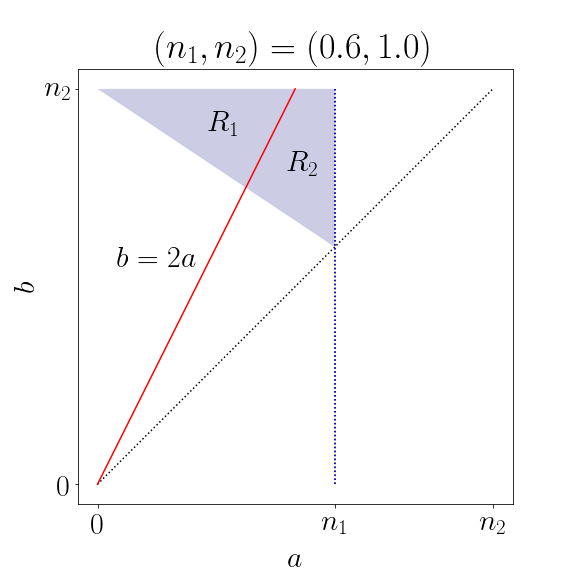
\includegraphics[width=.5\linewidth]{figures/fig4.png}
\end{figure}

The regions in the parameter space where oscillating spreading speed exists can be determined as follows: for any fixed choice of $(n_1,n_2)$, with $0<n_1<n_2$, let $R$ be the set of pairs $(a,b)\in\mathbf R^2$ such that the hypothesis of Theorem 2.1 holds. Then $R$ is a triangle in the $a$-$b$ plane with endpoints at $(0,n_2)$, $(n_1,n_1)$, and $(n_1,n_2)$, depicted in Figure \ref{fig:phaseportrait}. The line $b=2a$ partitions $R$ into two non-empty sets $R_1=\{(a,b)\in R:a\leq b/2\}$ and $R_2=\{(a,b)\in R:a> b/2\}$ such that the traveling has constant speed if $(a,b)\in R_1$ and oscillating speed if $(a,b)\in R_2$.


%\end{multicols}


\begin{thebibliography}{9}
\bibitem{all}  W. C. Allee. 1931. Animal Aggregations. A Study on
General Sociology. University of Chicago Press, Chicago, IL.


%\bibitem{htw90} D. P. Hardin, P. Tak$\acute{\mbox{a}}\check{\mbox{c}}$, and G. F. Webb. 1990. Dispersion population %models discrete in time and
%continuous in space. J. Math. Biol. {\bf 28}: 1-20.

\bibitem{hh} A. Hastings and K. Higgins. 1994. Persistence of transients in spatially
structured ecological models. Science {\bf 263}: 1133-1136.

%\bibitem{hz} S.-B. Hsu and X.-Q. Zhao. 2008. Spreading speeds and traveling waves for nonmonotone integrodifference equations. SIAM J. Math. Anal. {\bf} 40: 776–789


\bibitem{ks} M. Kot and W. M. Schaffer. 1986.  Discrete-time growth-dispersal models.
Math. Biosci. {\bf 80}: 109-136.


\bibitem{kot89} M. Kot. 1989. Diffusion-driven period doubling bifurcations.
Biosystems {\bf 22}: 279-287.


\bibitem{kot92} M. Kot. 1992. Discrete-time traveling waves:
Ecological examples. J. Math. Biol. {\bf 30}: 413-436.


\bibitem{kot1} M. Kot, M. A. Lewis, and P. van den Driessche. 1996. Dispersal data and the spread of invading
organisms. Ecology {\bf 77}: 2027-2042.


%\bibitem{kot2} M. Kot, J. Medlock, T. Reluga, and D. B. Walton. 2004. Stochasticity, invasions, and branching random walks. Theor. Popul. Biol. {\bf 66}: 175-184.


%\bibitem{li09} B. Li, M. A. Lewis, and H. F. Weinberger. 2009.  Existence of traveling waves for integral recursions with nonmonotone growth functions. J. Math. Biol. {\bf 58}: 323-338.


\bibitem{kotbook} M. Kot. 2001. Elements of Mathematical Ecology.
Cambridge University Press. Cambridge, United Kingdom.

\bibitem{lui82a} R. Lui. 1982. A nonlinear integral operator arising from a model in population
genetics. I. Monotone initial data. SIAM. J. Math. Anal. {\bf 13}:
913-937.

\bibitem{lui82b} R. Lui. 1982. A nonlinear integral operator arising from a model in population
genetics. II. Initial data with compact support. SIAM. J. Math.
Anal. {\bf 13}: 938-953.

\bibitem{lui83} R. Lui. 1983. Existence and stability of traveling wave solutions of a nonlinear
integral operator. J. Math. Biol. {\bf 16}:199-220.

\bibitem{lut}
F. Lutscher. 2019. Integrodifference Equations in Spatial Ecology.  Springer.


\bibitem{nkl} M. Neubert, M. Kot, and M. A. Lewis. 1995. Dispersal and pattern formation in a
discrete-time predator-prey model. Theor. Pop. Biol. {\bf 48}
: 7-43.

\bibitem{otto} G. Otto. 2017. Non-spreading Solutiona in a Integro-Difference Model Incorporating Allee and Overcompensation Effects. Ph. D thesis, University of Louisville.

\bibitem{slatkin} M. Slatkin. 1973. Gene flow and selection in a cline.
Genetice {\bf 75}: 733-756.



\bibitem{pnas} L. L. Sullivan, B. Li, T. E. X. Miller, M. G. Neubert, and A. K. Shaw. 2017.
Density dependence in demography and dispersal generates fluctuating invasion speeds. Proc. Natl. Acad. Sci. USA {\bf
114}: 5053-5058.


\bibitem{wang} M. H. Wang, M. Kot, and M. G. Neubert. 2002. Integrodifference equations, Allee effects, and
invasions. J. Math. Biol. {\bf 44}: 150-168.

\bibitem{w78} H. F. Weinberger. 1978. Asymptotic behavior of a model in  population genetics,
in Nonlinear Partial Differential Equations  and Applications, ed.
J. M. Chadam. Lecture Notes in Mathematics {\bf 648}: 47-96.
Springer-Verlag, Berlin.

\bibitem{wein82} H. F.  Weinberger. 1982. Long-time beahvior of a class of biological models. SIAM. J.
Math. Anal. {\bf 13}: 353-396.

\end{thebibliography}


\appendix

\section{Appendix}

%\begin{proof}[Proof of Proposition \ref{prop1}]
%
%Let $u(x)$ be non-negative, continuous, and bounded.
%
%\begin{enumerate}[(i.)]
%\item For $t\in\mathbb R$, let $T^t$ denote the translation operator defined $T^t[u](x) = u(x+t)$. Then,
%\begin{equation} \begin{aligned}
%Q[T^t[u]](x) &= 
%\int_{-\infty}^{\infty} k(x-y) g(T^t[u](y)) \, dy \\
%&= \int_{-\infty}^{\infty} k(x-y) g(u(y+t)) \, dy
%\end{aligned} \end{equation}
%Let $z=y+t$.
%\begin{equation} \begin{aligned}
%Q[T^t[u]](x)
%&= \int_{-\infty}^{\infty} k(x-z+t) g(u(z)) \, dz \\
%&= Q[u](x+t) \\
%&= T^t[Q[u]](x)
%\end{aligned} \end{equation}
%
%\item 
%Suppose $\lim_{x\to\infty}u(x)=\ell$. 
%
%\end{enumerate}
%
%\end{proof}

\begin{lem} \label{laplaceproof}
The Laplace kernel \eqref{laplacekernel} satisfies hypothesis (H4).
\end{lem}

\begin{proof}
Let $k(x)=\frac{1}{2}e^{-|x|}$. For $a \in \mathbb R$ and $\lambda \in (0,1)$, define
\begin{equation}
f_{a,\lambda}(x)= \frac{1}{2} e^{-|x|} - \frac{\lambda}{2}e^{-|x-a|}.
\end{equation}

If $a=0$, then $f$ has no zero-crossings, since $f_{0,\lambda}(x)=\frac{1-\lambda}{2}e^{-|x|}$ is strictly positive. If $a$ is nonzero, then one can easily check the symmetry relation $f_{-a,\lambda}(x)=f_{\lambda,a}(-x)$. Since the number of zero-crossings are invariant with respect to a reflection about the vertical axis, we can assume without loss of generality $a>0$.

Under this assumption, $f$ is strictly increasing on $(-\infty,0)$, and strictly decreasing on $(0,a)$. The behavior on $(a,\infty)$ can be determined in three cases:

\begin{enumerate}[{Case} 1.)]
\item if $a<\ln\frac{1}{\lambda}$, then $f$ is decreasing on $(0,\infty)$, hence has no zero-crossings;
\item if $a>\ln\frac{1}{\lambda}$, then $f$ has a unique zero-crossing at $x=\frac{1}{2}(a-\ln\lambda)$;
\item if $a=\ln\frac{1}{\lambda}$, then $f$ vanishes on $(a,\infty)$, hence it has no zero-crossings.
\end{enumerate}
In each case, the number of zero-crossings does not exceed one.
\end{proof}

\begin{lem}\label{laplacebound}
If $k(x)$ is given by the Laplace kernel, then $w_1$ and $w_2$ form a periodic traveling wave solution if $C_1\leq 0$, or if $C_1>0$ and $w_2\left(\ln\sqrt\frac{C_3}{C_2}\right)\leq b$.
\end{lem}

\begin{proof}
We can proceed in cases. If $C_1\leq 0$, then $w_2(x)$ is monotone decreasing, hence $w_2(x)<w_2(-\infty)=m<b$ everywhere. Otherwise, if $C_1>0$, then $w_2(x)$ is increasing on $(-\infty,\beta)$ and decreasing on $(\alpha,\infty)$. Since $w_2(x)$ is concave-down on $(\beta,\alpha)$, this implies there is a unique global maximum somewhere in this interval. To find it, we can differentiate:
$$ \frac{dw_2}{dx}\Big|_{\beta<x<\alpha}=C_3e^{-x}-C_2e^x $$
Setting this expression equal to zero and multiplying by $e^x$, we obtain $C_3-C_2e^{2x}=0$, which has a unique solution at $x=\ln\sqrt\frac{C_3}{C_2}$.
\end{proof}

\begin{lem}
The Gaussian kernel satisfies hypothesis H4.
\end{lem}

\begin{proof}
Let $a\in\mathbb R$ and $\mu\in(0,1)$. Then
\begin{equation} \begin{aligned}
k(x)-\mu k(x-a) &= \frac{1}{\sqrt{2\pi}} \left( e^{-\frac{x^2}{2}} - \mu e^{-\frac{-(x-a)^2}{2}} \right) \\
&= \frac{1}{\sqrt{2\pi}} e^{-\frac{x^2}{2}} \left( 1 - \mu e^{\frac{2ax-a^2}{2}} \right)
\end{aligned} \end{equation}
This expression has a unique zero at $x=\frac{y^2-2\ln(\mu)}{2a}$, so the number of zero-crossings is at most one.
\end{proof}

\begin{lem}
For the Gaussian kernel, $w_2(x)$ has a unique local extrema which is a global maxium at $x=\frac{2\ln(1-m)}{\alpha-\beta}+\alpha+\beta$.
\end{lem}

\begin{proof}
The derivative of $w_2(x)$ is given by
$$ 
\frac{dw_2}{dx} = -\frac{1}{\sqrt{2\pi}}e^{-\frac{(x-\alpha)^2}{2}} + \frac{1-m}{\sqrt{2\pi}}e^{-\frac{(x-\beta)^2}{2}}
$$
Setting this quantity equal to zero, we obtain the equation
$$ 
e^{-\frac{(x-\alpha)^2}{2}} = (1-m)e^{-\frac{(x-\beta)^2}{2}}
$$
Taking logarithm on both sides, and rearrange terms,
$$ 
(x-\beta)^2 = 2\ln(1-m) + (x-\alpha)^2
$$
Distributing both sides and cancelling the quadratic term, we get the solution
$$
x = \frac{2\ln(1-m)}{\alpha-\beta} + \alpha + \beta
$$
\end{proof}

\end{document}

